\documentclass{article}
\usepackage{graphicx} % Required for inserting images
\usepackage[utf8]{inputenc}
\usepackage[vietnam]{babel}
\usepackage{amsmath}
\usepackage{graphicx}
\usepackage{hyperref}
\usepackage{geometry}
\usepackage{titling}
\usepackage{lmodern} 
\usepackage{diagbox}
\usepackage{placeins}
\usepackage{float}
\usepackage{fontawesome5}


\usepackage{listings}
\usepackage{color}

\definecolor{keywordcolor}{rgb}{0.13, 0.29, 0.53}
\definecolor{commentcolor}{rgb}{0.34, 0.53, 0.21}
\definecolor{stringcolor}{rgb}{0.63, 0.25, 0.44}

\lstset{
    basicstyle=\ttfamily,
    keywordstyle=\color{keywordcolor}\bfseries,
    commentstyle=\color{commentcolor}\itshape,
    stringstyle=\color{stringcolor},
    showstringspaces=false,
    frame=single,
    breaklines=true,
    numbers=left,
    numberstyle=\tiny,
    numbersep=5pt,
}

% Page setup
\geometry{margin=1in}

% Title and authors
\title{AI002.P11 Final Report,\\Artificial Intelligence Thinking PhD. Ngo Duc Thanh,\\Group 16,\\ English vocabulary recommendation for learning}
\author{
    Nguyen Tran Nhat Trung \\
    \small 23521684
    \and Pham Hai Dang \\
    \small 23520233
    \and Hoang Hai Duong\\
    \small 23520345
}
\date{January 26, 2025}

\begin{document}
% Title page
\maketitle

% Abstract
\begin{abstract}
This project introduces an approach to English vocabulary (\textit{e.g. flashcard, question,...}) recommendation \textit{for learning} by leveraging the BEIT3 model for text embeddings and integrating the Oxford Dictionary as a source of word-definition pairs. The BEIT3 model, a state-of-the-art text-to-text foundation model, is employed to calculate embeddings of word definitions, enabling semantic representation of vocabulary in a dense vector space. Our methodology enhances personalization by incorporating contextual data such as user hobbies, career aspirations, and web search history, which are embedded into the same vector space. This personalization ensures the recommendation of words that are not only semantically related but also contextually relevant to the user's interests and needs.
\end{abstract}

\tableofcontents
\newpage


\section{Problem statement}
\subsection{Input:}
\begin{itemize}
    \label{sec:input1}
    \item \textbf{User provided information\hyperref[sec:input1]{[d1]}}: such as \textbf{age}, \textbf{occupation}, \textbf{hobbies}, \textbf{interests}, and \textbf{gender}, is processed through a detailed feature extraction pipeline to ensure structured and actionable insights. 
    \textbf{Age} is represented numerically (e.g., 18), or can be describe as text as categories such as "young", "adult" or "senior". \textbf{Occupation} titles are standardized into broader categories or just a title of job (e.g., "Technology", "Engineer").  \textbf{Hobbies} are text describe user's hobbies (e.g., "Football", "Sports"). \textbf{Interests} are things that users frequently view and like, from which we can know their needs (e.g., "Political", "Gaming news"). \textbf{Gender} is a string so that can be used by people in specific community and culture (e.g., "Male", "Female"). For example:
    \begin{figure}[h!]
        \centering
        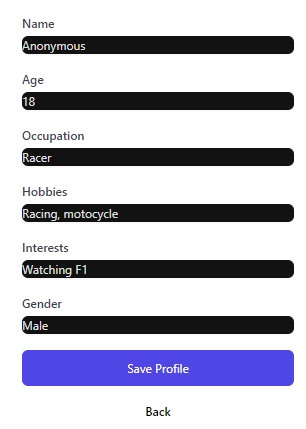
\includegraphics[width=0.3\linewidth]{user-profile.png}
        \caption{User's provided infomation example}
        \label{fig:enter-label}
    \end{figure}
    \label{sec:input2}
    \item \textbf{User's learning data\hyperref[sec:input2]{[d2]}:} User learning data comprises the user's \textbf{word\_id}, the \textbf{score} they obtained, and the \textbf{time} at which that score was achieved. This data is instrumental in calculating \textit{penalties}, which in turn enhances the diversity and effectiveness of flashcard recommendations. By analyzing user performance over time, the system can identify areas where the user may need additional practice and tailor the flashcards accordingly. This personalized approach can significantly improve learning outcomes. This data will be filled automatically during the learning process. For example:
    \begin{figure}[h!]
        \centering
        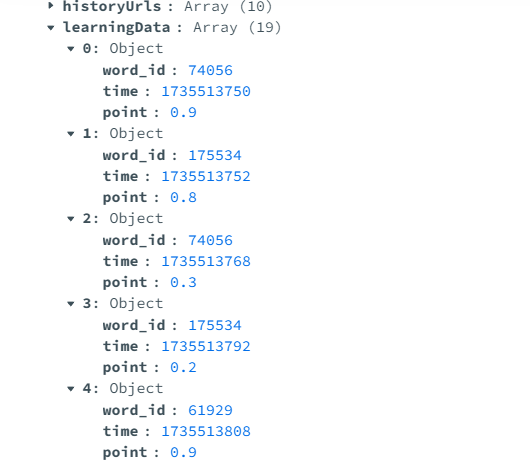
\includegraphics[width=0.3\linewidth]{user-learning-data.png}
        \caption{User's learning data example}
        \label{fig:enter-label}
    \end{figure}
    \label{sec:input3}
    \item \textbf{User's browser history: }The URLs (\textit{strings}) obtained from the user's browsing history constitute a valuable data for the application's recommendation system, enabling it to discern the user's interests through techniques such as URL parsing, topic modeling, and collaborative filtering, ultimately facilitating the provision of highly personalized and engaging content recommendations. This input will automatically \textbf{track} from the browser. For example:
    \begin{figure}[h!]
        \centering
        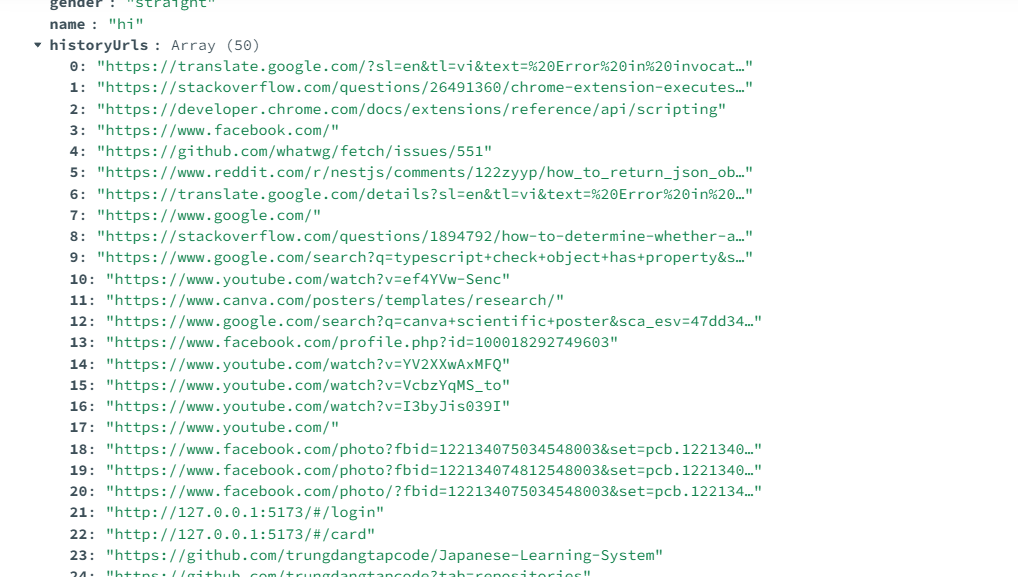
\includegraphics[width=0.5\linewidth]{user-browser-history.png}
        \caption{User's browser history example}
        \label{fig:enter-label}
    \end{figure}
    \label{sec:input4}
    \item \textbf{User's translated text: }is a literal "corpus" of English words that users have translated. We developed a \textit{small browser extension} that facilitates seamless text translation while users browse the web or read online articles. This extension automatically captures and stores translated text into the \textit{local storage}, creating a personalized dataset that highlights areas where users face linguistic challenges. The \textbf{automated} storage mechanism ensures the translation history is continuously updated, enabling the system to adaptively track and address the user's learning needs. For example:
\begin{figure}[h!]
    \centering

    \begin{minipage}{0.45\textwidth}
        \centering
        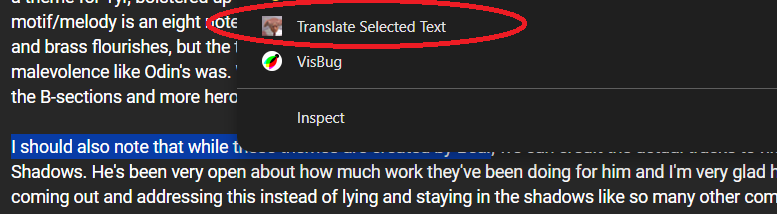
\includegraphics[width=\textwidth]{translated-text-example-1.png}
        \caption{Translated text example (built-in extension)}
        \label{fig:enter-label}
    \end{minipage}
    \begin{minipage}{0.45\textwidth}
        \centering
        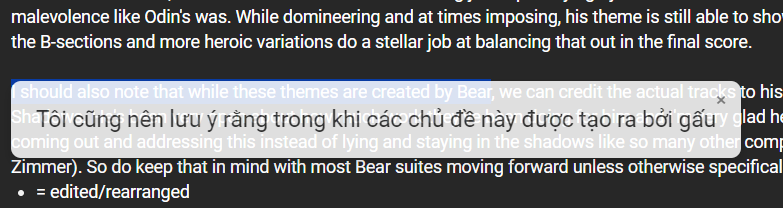
\includegraphics[width=\textwidth]{translated-text-example-2.png}
        \caption{Translated text example (after translating, save the English text)}
        \label{fig:enter-label}
    \end{minipage}
\end{figure}
    \begin{figure}[h!]
        \centering
        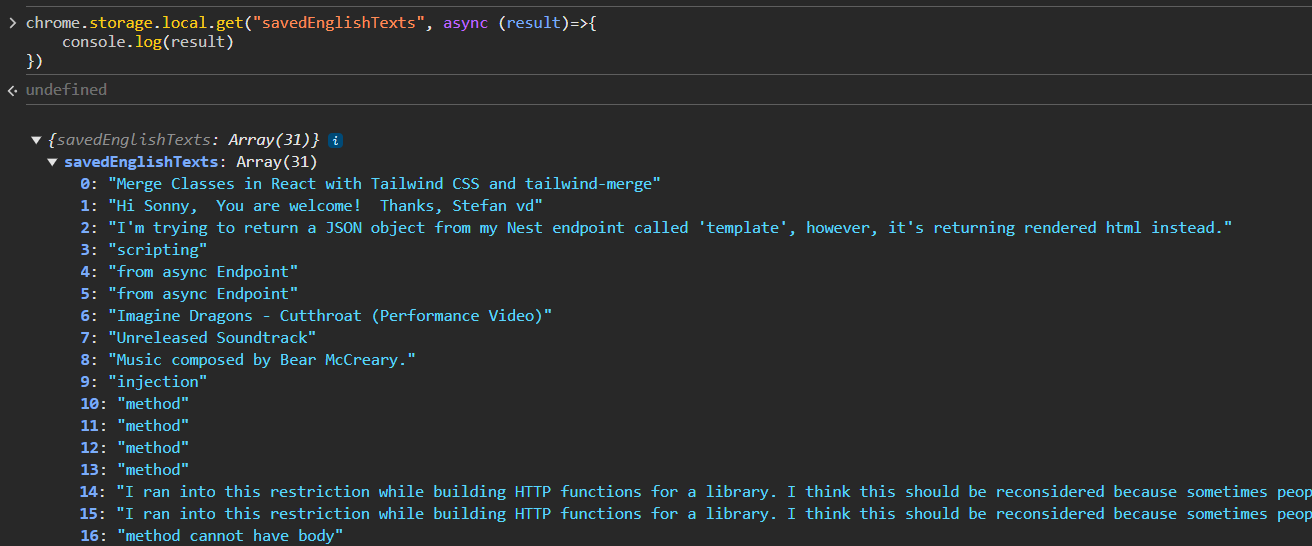
\includegraphics[width=0.5\linewidth]{translated-text-example-3.png}
        \caption{Translated text example (the translated text saved on local storage of chrome)}
        \label{fig:enter-label}
    \end{figure}
    \item \textbf{Dictionary data (optional): }it refers to a structured repository of terms, definitions. It functions as a corpus that supports retrieval operations, enabling the generation of relevant flashcards based on user queries or knowledge gaps. For example:
    \begin{figure}[h!]
        \centering
        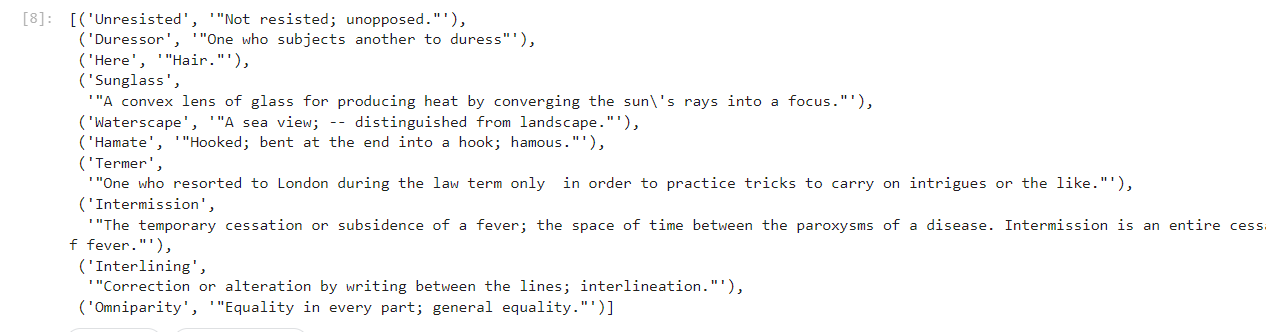
\includegraphics[width=0.75\linewidth]{dictionary-example.png}
        \caption{Dictionary data example}
        \label{fig:enter-label}
    \end{figure}
\end{itemize}
\label{sec:input10}
\subsection{Output\hyperref[sec:input10]{[d10]}}
A \textit{single} object is the question with four possible answer choices, only one of which is correct (also the index for the correct one). To ensure variety and prevent memorization of specific card orders, the system employs a \textbf{randomized} output mechanism. This means that given the same user data and information retrieved from the database, the specific question presented on a flashcard may vary across different sessions or even within the same session. However, the system is designed to prioritize the presentation of flashcards that are most relevant and beneficial to the user's learning progress. This prioritization is achieved through a probabilistic approach, where flashcards that address the user's areas of weakness or align with their learning objectives are more likely to be presented. This dynamic and adaptive approach enhances the learning experience by continuously challenging the user and providing a personalized learning path.

\begin{figure}[h!]
    \centering

    \begin{minipage}{0.45\textwidth}
        \centering
        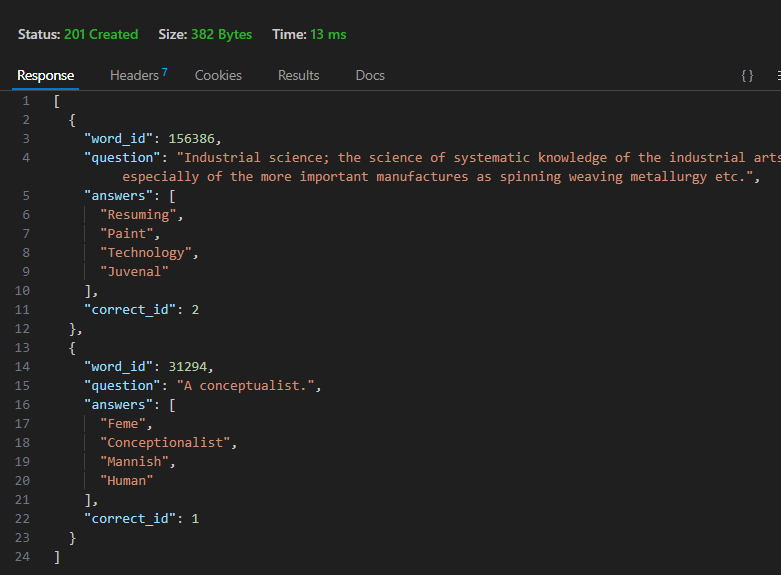
\includegraphics[width=\textwidth]{output-backend.png}
        \caption{Output example (backend)}
        \label{fig:enter-label}
    \end{minipage}
    \begin{minipage}{0.45\textwidth}
        \centering
        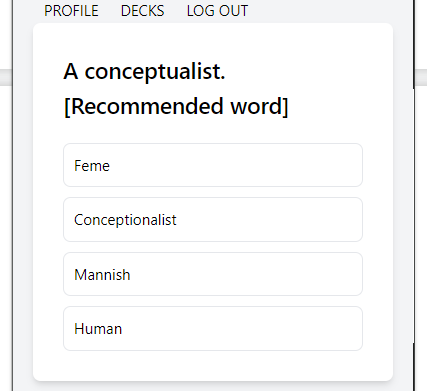
\includegraphics[width=\textwidth]{output-frontend.png}
        \caption{Output example (frontend)}
        \label{fig:enter-label}
    \end{minipage}
\end{figure}

\subsection{Constraint:}
\begin{enumerate}
    \item \textbf{Information as English Text}  
    \begin{itemize}
        \item \textbf{Constraint:} All input information provided by the user must be in English text.
        \item \textbf{Reason:} Since the vocabulary recommendation system is built upon English text processing and embeddings generated by the BEIT3 model, using English ensures compatibility and accurate feature extraction. Non-English input could introduce errors or inconsistencies in the recommendation process.
        \item \textbf{Impact:} This constraint ensures that the system can effectively process the user’s input, whether it’s their hobbies, career details, or translations, and generate meaningful vocabulary suggestions tailored to their needs.
    \end{itemize}
    
    \item \textbf{Information Needs to Be Honest}  
    \begin{itemize}
        \item \textbf{Constraint:} Users must provide honest information about their interests, career, hobbies, and other details.
        \item \textbf{Reason:} The accuracy and personalization of the recommendations rely heavily on the quality of the user-provided data. If the information is dishonest or inaccurate, the system may recommend irrelevant vocabulary, undermining its effectiveness and reducing the user’s satisfaction.
        \item \textbf{Impact:} Honest data enables the system to better align vocabulary recommendations with the user’s goals, making the learning process more effective and relevant to their context.
    \end{itemize}
    
    \item \textbf{Chrome Extension to Access Browser History}  
    \begin{itemize}
        \item \textbf{Constraint:} The application must have access to the user’s browser history through a Chrome extension.
        \item \textbf{Reason:} Browser history provides valuable contextual data about the user’s online activities, such as websites visited and topics of interest. Extracting metadata like keywords from URLs enables the system to recommend vocabulary that aligns with the user’s browsing habits.
        \item \textbf{Impact:} By leveraging browser history, the system can identify frequently visited topics and domains, ensuring the recommended vocabulary is not only personalized but also practical for the user’s everyday use.
    \end{itemize}
\end{enumerate}


    
\subsection{Requirement:}


\begin{enumerate}
    \item \textbf{Diverse Recommendations:}  
    The vocabulary recommendations should exhibit a high level of diversity to ensure users are exposed to a broad range of words.  
    \begin{itemize}
        \item Diversity is measured using the \textbf{Type-Token Ratio (TTR)\hyperref[sec:TTR]{[3.1]}}.
        \item \textbf{Requirement:} The TTR for the recommended vocabulary set must be greater than \textbf{0.7}.
        \item \textbf{Reason:} A higher TTR ensures that the recommended words are unique and reduce redundancy, making the learning process more engaging and effective.
    \end{itemize}
    
    \item \textbf{Positive User Feedback:}  
    The system must prioritize recommendations that align with the user’s preferences and learning experience.
    \begin{itemize}
        \item Users rate the recommended vocabulary on a scale of 1 to 5. Helps to improve the user's score during the learning process, which is calculated as in \hyperref[sec:confidence-score]{[3.2]}.
        \item \textbf{Requirement:} A word is considered successfully recommended if the user gives it a rating of \textbf{3 or higher}.
        \item \textbf{Reason:} This ensures that the system is actively refining its recommendations to match the user’s needs and preferences based on feedback.
    \end{itemize}
    
    \item \textbf{Efficient Retrieval and Response Time:}  
    The application must be optimized for fast processing and response.
    \begin{itemize}
        \item \textbf{Requirement:} The total time for vocabulary retrieval and server response must not exceed \textbf{5 seconds}.
        \item \textbf{Reason:} A quick response time ensures a seamless user experience and minimizes frustration caused by delays, encouraging consistent use of the application.
    \end{itemize}
\end{enumerate}

\noindent \textbf{Summary of Requirements:}  
These requirements are designed to balance \textbf{effectiveness}, \textbf{user satisfaction}, and \textbf{system performance}. By ensuring diversity through TTR, aligning recommendations with user feedback, and maintaining quick response times, the system can deliver a high-quality personalized learning experience.


\section{Decomposition}
In designing a flashcard recommendation system, the problem can be decomposed into two perspectives: aggregation and individual diversity. From the aggregation perspective, the goal is to ensure that the recommendation system covers a wide range of topics across all users, promoting comprehensive coverage of the flashcard database. This is particularly useful in collaborative learning environments where diverse content exposure is beneficial. On the other hand, the individual perspective focuses on tailoring recommendations to maximize the balance between quality and diversity for a specific user. Here, the system should optimize for relevance by prioritizing flashcards that address the user's current learning goals while introducing new or less familiar topics to enhance learning breadth. Achieving this trade-off requires personalized algorithms that adapt to a user’s progress and preferences, ensuring effective and diverse learning experiences.To address these dual perspectives, the problem can be decomposed into the following steps: 

\begin{figure}[h!]
    \centering
    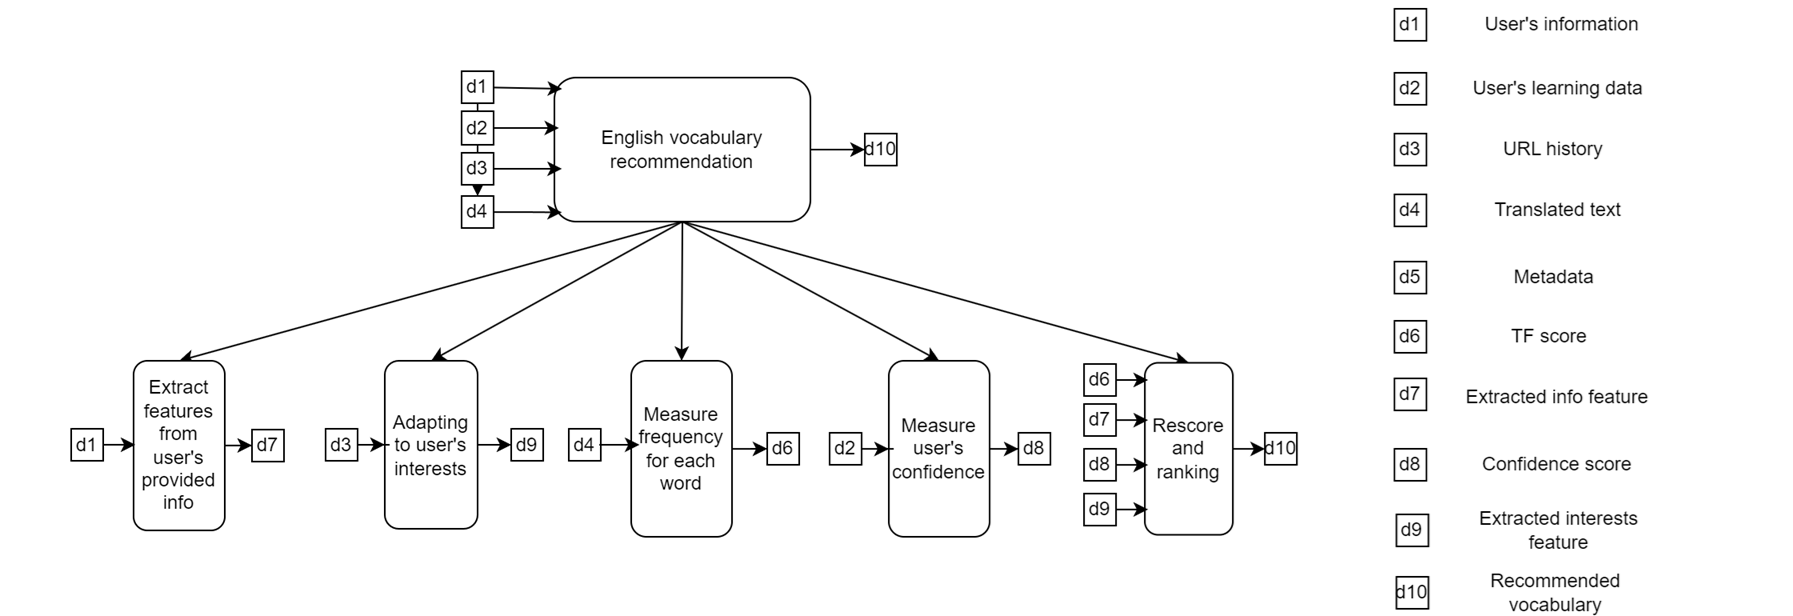
\includegraphics[width=0.9\linewidth]{decomposition-tree.png}
    \caption{Decomposition Tree}
    \label{fig:decomposition-tree}
\end{figure}

\subsection{Extract features from user's provided info}
\begin{itemize}
    \item \textbf{Input\hyperref[sec:input1]{[d1]}:} The user's provided data, which includes key demographic and behavioral attributes such as age, occupation, hobbies, interests, and gender. This raw input serves as the foundation for deriving actionable insights and generating personalized outputs.
    \label{sec:input7}
    \item \textbf{Output\hyperref[sec:input7]{[d7]}:} The extracted feature that represent the input information in a machine-readable format. These features are tailored to encapsulate the user's profile in a way that can be leveraged by downstream algorithms or recommendation systems.
\end{itemize}
The core focus of this project lies in addressing the challenge of acquiring user-provided information, processing it into semantic embedding vectors, and subsequently leveraging these embeddings to generate tailored flashcard content. This solution aims to enhance user engagement and learning outcomes by providing content that is semantically aligned with user input. A detailed depiction of the semantic embedding process is illustrated in \ref{fig:decompose1-embedding-bio}, which outlines the multi-step transformation of raw input into meaningful vector representations.

\begin{figure}[h!]
    \centering
    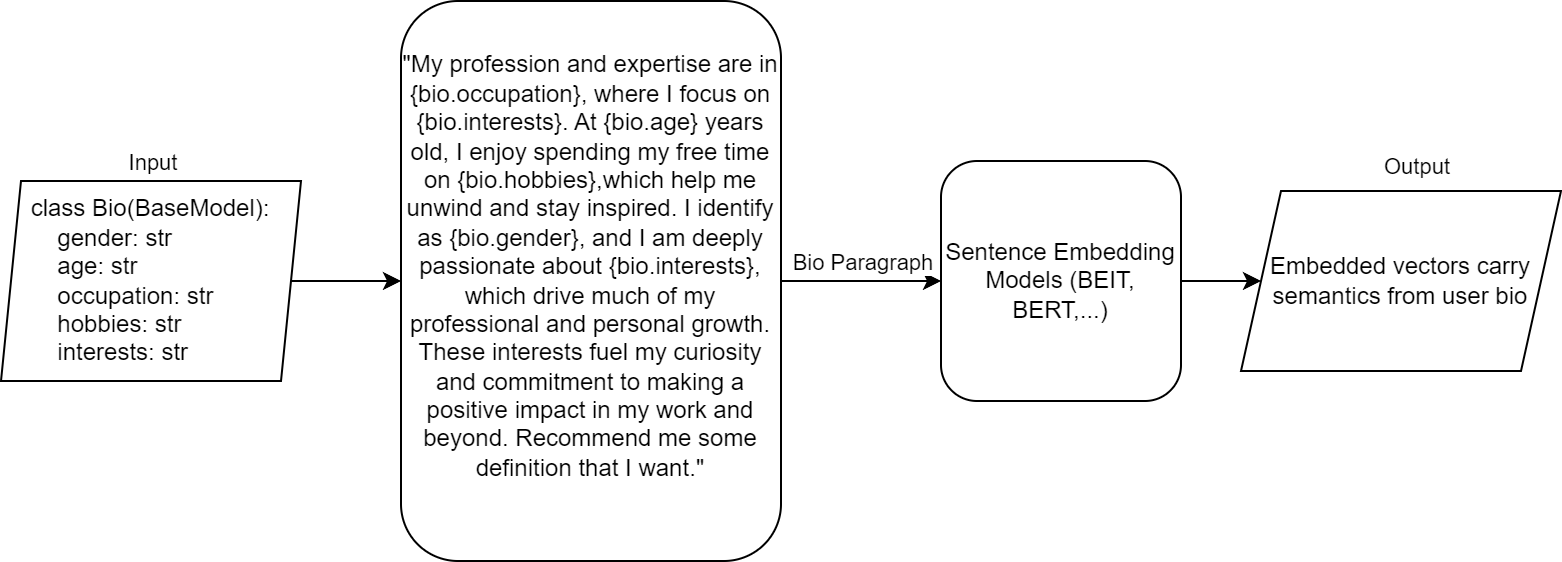
\includegraphics[width=0.8\linewidth]{decompose1-embedding-bio.png}
    \caption{Extract features from user's provided info}
    \label{fig:decompose1-embedding-bio}
\end{figure}

To achieve high-quality embeddings, we experimented with various deep learning models while maintaining consistent system hyperparameters, such as batch size, learning rate, optimizer configuration, and evaluation metrics. The performance outcomes of these models are summarized in \ref{table:beit-bert}. Through rigorous comparative analysis, the BEIT model emerged as the optimal choice. Its ability to generate robust contextualized representations made it a standout among competing architectures. The BEIT model's effectiveness stems from its transformer-based architecture, originally designed for image processing, which we adapted for text-based semantic embeddings. Its self-attention mechanism captures long-range dependencies, ensuring the creation of high-dimensional embeddings that encapsulate nuanced semantic information.

\FloatBarrier
\begin{table}[H]
\centering
\begin{tabular}{|p{0.5\textwidth}|p{0.2\textwidth}|p{0.2\textwidth}|}
\hline
\diagbox[width=\dimexpr \textwidth/8+4\tabcolsep\relax, height=1cm]{ Person }{Model (r-5)} & BEIT & BERT \\ \hline
Person A:
\{gender: "male", age: "20", 
occupation: "game developer", 
hobbies: "playing game", 
interests: "news about game, developing"\}        
& Game Development, Gaming, News, Developer, Programming      
& Modeling, Tech, Gamer,  Updates, Design      \\ \hline
Person B:
\{gender: "female",
age: "20",
occupation: "Artist",
hobbies: "Painting, sketching",
interests: "Art trends, creative techniques, art exhibitions"& 
Art, Creativity, Painting, Sketching, Artist      & 
Trends, Expression, Design, Exhibitions, Note     \\ \hline
\end{tabular}
\caption{Compare BEIT and BERT on recommending word}
\label{table:beit-bert}
\end{table}

\subsection{Adapting to user's interests}
\begin{itemize}
    \item \textbf{Input\hyperref[sec:input3]{[d3]}:} URLs from analyzing the websites user visit. We can understand their interests. This allows us to suggest relevant and engaging content, creating a more personalized experience. This browsing information will be automatically collected from the user's browser
    \label{sec:input9}
    \item \textbf{Output\hyperref[sec:input9]{[d9]}:} The extracted features represent the input information in a machine-readable format. These features are tailored to encapsulate the user's history in a way that can be leveraged by downstream algorithms or recommendation systems.
\end{itemize}

The system must track the user's browsing data in real-time, responding to every change in the user's search history. This requires implementing a browser extension or script capable of detecting URL changes (through \textit{onHistoryStateUpdated}). Each detected change needs to be communicated to the backend promptly, ensuring minimal latency and synchronization between the front-end tracker and the back-end processor. For example, when a user navigates from \textit{example.com} to \textit{news.com}, this transition must be recorded and transmitted efficiently.

The URLs must be analyzed and filtered to remove invalid or irrelevant entries, such as dynamically generated tracking links, advertisements, or non-content URLs (e.g., authentication pages or error pages). This step necessitates employing a robust URL validation mechanism and possibly integrating a domain categorization service to identify valid content-rich sources. For instance, retaining en.wikipedia.org/wiki/Machine\_learning would ensure relevant data is processed. And here some invalid URL:

\begin{table}[H]
\centering
\begin{tabular}{|p{0.4\textwidth}|p{0.45\textwidth}|}
\hline
Invalid URL & Reason \\
\hline
http://localhost:8080 &
These URLs are only accessible within a specific network and aren't accessible from outside the local environment. \\
\hline
https://example.com/app\#fragment &
If the metadata is generated dynamically via JavaScript, tools that don't execute JavaScript (e.g., simple crawlers or requests in Python) will not be able to retrieve it. \\
\hline
https://nonexistentdomain12345.com &
If the URL points to a domain or resource that no longer exists, metadata retrieval will fail. \\
\hline
https://securewebsite.com/private-area &
If the URL requires authentication (e.g., Facebook account) to access, metadata retrieval will fail without proper credentials.\\
\hline
\end{tabular}
\caption{Example of Invaid URL}
\label{table:invalid-url}
\end{table}

For each valid URL, the system must retrieve metadata such as the webpage title, description, and keywords. This involves parsing the website's HTML using web scraping or metadata extraction tools and ensuring compliance with web crawling guidelines

\begin{table}[H]
\centering
\begin{tabular}{|p{0.3\textwidth}|p{0.2\textwidth}|p{0.2\textwidth}|p{0.2\textwidth}|}
\hline
URL & Title & Description & Keywords \\
\hline
{\raggedright
https://www.freecodecamp.org/
news/ai-in-agriculture-book/
\par
}
&
AI in Agriculture: How AI-Enhanced Farming Can Increase Crop Yields [Full Book]
&
Artificial intelligence is revolutionizing the agriculture industry, paving the way for a future of smarter, more efficient farming practices. Imagine a world where crops are grown with precision and care, maximizing yields like never before. With AI...	
&
Artificial intelligence, future, machine learning
\\
\hline
https://www.youtube.com/ watch?v=66fXm8lfOLE
&
Ban tin UIT News thang 1/2025 | UIT RON RANG DON NAM MOI XUAN AT TY 2025 - YouTube
&
Thang 1, Truong Dai hoc Cong nghe Thong tin co nhung noi dung noi bat nhu sau:- KY HOP HOI DONG TRUONG DAI HOC CONG NGHE THONG TIN LAN THU 17 (KHOA I) - LE CO...
&
video, sharing, camera phone, video phone, free, upload\\
\hline
\end{tabular}
\caption{Example of Metadata of URL}
\label{table:metadata-url}
\end{table}

The extracted metadata must be converted into a numerical embedding vector that semantically represents the content.The embeddings from multiple URLs are then aggregated using an Exponentially Weighted Moving Average (EWMA) mechanism, emphasizing recent browsing behavior while retaining the influence of past activities. For example, if the user visits websites related to "Data Science" followed by "Machine Learning," the aggregated embedding should gradually shift towards representing their evolving interests. This pipeline not only requires seamless integration across multiple components but also demands computational efficiency and scalability to handle diverse and dynamic browsing behaviors. 
\begin{align*}
\mathbf{s}_t &\leftarrow \alpha \mathbf{v}_t + (1 - \alpha) \mathbf{s}_{t-1} \\
\mathbf{s}_{corrected} &\leftarrow \frac{s_t}{1-\alpha^t}
\end{align*}

\text{Where:}
\begin{itemize}
    \item $\mathbf{s}_{t}$, $\mathbf{s}_{t-1}$ is the EWMA vector at time $t$, $t-1$.
    \item $\mathbf{v}_t$ is the input vector at time $t$ (feature extracted new URL).
    \item $\alpha$ (where $0 < \alpha \leq 1$) is the smoothing factor that determines the weight given to recent versus past observations.
\end{itemize}

\subsection{Measure frequency for each word.}
\begin{itemize}
    \item \textbf{Input\hyperref[sec:input4]{[d4]}:} is a "corpus", is a concatenated string derived from the translatedText field within a data comprising user-generated translations. 
    \label{sec:input6}
    \item \textbf{Output\hyperref[sec:input6]{[d6]}:} is a frequency distribution of words within the vocabulary. Specifically, for each unique word in the corpus, the output should provide its \textit{Term Frequency (TF)} score. The overarching objective is to identify the words that exhibit the highest frequency within user-generated translations, thereby pinpointing the vocabulary items that users consistently encounter and potentially struggle with.
\end{itemize}

A challenge here is ensuring that the data is clean and uniform, as user-translated sentences often contain inconsistencies like extra spaces, punctuation errors, and variations in word case. These inconsistencies can skew the term frequency (TF) calculations. 
For example, consider users translate sentences such as:
\begin{itemize}
    \item "The cat sat on the mat."
    \item "A CAT sat on the mat!"
    \item These sentences, when concatenated, produce the corpus: "The cat sat on the mat. A CAT sat on the mat!". Preprocessing should include normalization (e.g., converting to lowercase), tokenization (splitting into words), and removal of stopwords (e.g., "the", "on", "a"). After preprocessing, the corpus becomes: "cat sat mat cat sat mat".
\end{itemize}
To solve this, develop a preprocessing pipeline that normalizes the data, splits it into tokens, and removes irrelevant terms. Tools like \textit{nltk} or \textit{spaCy} (in Python) can automate this process.

Once the corpus is preprocessed, the next task is to create a vocabulary—a set of unique words. This is crucial for calculating the TF score, as each word in the vocabulary needs to be assigned a score. A naive approach would be to extract every unique token from the corpus. 

For example, if the processed corpus is "cat sat mat cat sat mat", the vocabulary is {"cat", "sat", "mat"}. Tools like Python’s collections.Counter can help generate this vocabulary efficiently. To refine the vocabulary further, consider excluding words with low document frequency across users, as they contribute little to the goal of identifying common translation difficulties.

Then, we compute the TF score - it quantifies how frequently each word appears in the corpus relative to the total number of words. The formula for TF is
\[
TF(\omega)= 
\frac{
\text{Number of occurrences of $\omega$}
}{
\text{Total number of words in the corpus}
}
\]

This metric provides insight into which words users often translate, indirectly revealing the words they encounter frequently. For example, in the corpus \textit{"cat sat mat cat sat mat mat"}, the total word count is 6. The TF scores are calculated as follows:

\begin{itemize}
    \item For "cat": $TF=\dfrac{2}{7}=0.29$
    \item For "sat": $TF=\dfrac{2}{7}=0.29$
    \item For "mat": $TF=\dfrac{3}{7}=0.43$
\end{itemize}

The final step is to integrate the calculated TF scores into a recommendation system. Words with high TF scores are \textbf{prioritized}, as they are likely to indicate translation difficulties. You might combine the TF score with other metrics, such as user error rates or context-specific difficulty, to produce a comprehensive recommendation score.

\subsection{Measure user's confidence.}
\begin{itemize}
    \item \textbf{Input\hyperref[sec:input2]{d2}: }User learning data, including list of word\_ids, scores, and timestamps, informs penalty calculations to enhance flashcard recommendations. By analyzing performance trends, the system identifies areas needing improvement and adapts flashcards for effective learning.
    \label{sec:input8}
    \item \textbf{Output\hyperref[sec:input8]{d8}: }is structured as a dictionary, where each word\_id is associated with a confidence\_score that reflects the user’s current proficiency level with the corresponding vocabulary flashcard. A higher confidence\_score indicates greater familiarity or mastery of the word, thereby reducing the likelihood of its recommendation in subsequent practice sessions. This scoring mechanism ensures an adaptive learning experience, prioritizing words that require more attention while gradually phasing out those already mastered. The calculation of the final scores from the input will be discussed based on the formula in the section \ref{sec:confidence-score}.
\end{itemize}

\subsection{Rescore and ranking.}
\begin{itemize}
    \item \textbf{Input:} The input is the aggregation of the outputs of the above parts including: Extracted info feature\hyperref[sec:input7]{[d7]}, extracted interests feature\hyperref[sec:input9]{[d9]}, TF Score\hyperref[sec:input6]{[d6]}, confidence score\hyperref[sec:input8]{[d8]}.
    \item \textbf{Output\hyperref[sec:input10]{[d10]}: }generated flashcard where each card presents a single question with four possible answer choices, only one of which is correct.  
\end{itemize}

The recommendation task involves determining the most relevant word and its corresponding definition based on a set of outputs of subproblems. This problem is modeled as a weighted combination of vector embeddings, further refined by term frequency (TF) scores and penalized using confidence scores. Given two input vectors, $v_{bio}$\hyperref[sec:input7]{[d7]}, ${s}_{corrected}$\hyperref[sec:input9]{[d9]}, derived from distinct sources or contexts, we compute a weighted combination to form a single representative vector:
\[
    v_c = w_{bio}v_{bio}+w_{history}{s}_{corrected}
\]
where $w_{bio}, w_{history}$ are scalar weights that control the influence of each input vector. The weights can be tuned manually or learned through optimization techniques depending on the specific application. 
Then each word and its definition in \textit{vocabulary} are embedded into the same vector space using same model. The cosine similarity between the combined vector $v_{c}$ and the feature vector of a candidate word $\omega$ is $v_{\omega}$ (and its associated definition) is computed to measure semantic relevance.

To account for the importance of frequently occurring terms, a term frequency ($TF$) score is added as a bonus to the cosine similarity score. Let $TF_\omega$ denote the $TF$ score for a candidate word $\omega$. The adjusted score will be added a \textit{penalty} called confidence scores - it's represent the uncertainty in the input data. A higher confidence score indicates greater uncertainty and requires penalization. Previously we used Reciprocal Rank Fusion (RRF) but it is discretized by rank, losing the continuous meaning of similarity. The final score for each candidate is computed as:
\[
FinalScore_\omega = \left[Similarity(v_c,v_{\omega})+w_{TF}TF_{\omega}\right]\cdot e^{-\frac{confidence_\omega}{\tau_{conf}}}
\]

After the experiment, we decided to choose the default hyperparameters of the system as follows:

\begin{table}[H]
\centering
\begin{tabular}{c|c}
Hyperparameter& Value\\
\hline
$alpha$ & 0.1 \\
$w_{bio}$ & 0.6 \\
$w_{history}$ & 0.4 \\
$w_{TF}$ & 2.0 \\
$\tau_{conf}$ & 86400 \\

\end{tabular}
\caption{Default hyperparameter}
\label{table:hyperparameter}
\end{table}

\section{Evaluation}
The assessment of the system arises due to the fact that it is based on human interaction and is therefore dynamic, not static. Because the system runs in real-time, user-interactive mode, it cannot be evaluated like traditional systems using predefined, fixed datasets. For that reason, traditional evaluation methods which rely on static data cannot be applied here. Rather, the performance of this system has to be assessed using controlled experiments and a bunch of iterative tests that mimic actual usage situations. 

These tests are meant to show how well the system works in real life, concentrating on the user and the flexibility of the suggestions. The measuring steps are also organized by a list of clear goals that look at different parts of the system, like how right the recommendations are, how much users get involved, and what learning results come from using the suggested flashcards. Apply all these test methods and metrics of performance to give an evaluation that will be close to reality for the system, in terms of vocabulary improvement. Below are the metrics to evaluate the effectiveness of the system:

\subsection{Type-Token Ratio (TTR)}
\label{sec:TTR}
Type-Token Ratio (TTR) is a measure of lexical diversity in a set of recommended vocabulary. It is calculated as the ratio of unique words (types) to the total number of words (tokens) in a dataset. A higher TTR indicates a more diverse and varied vocabulary, while a lower TTR suggests repetition and limited variety.

In our context, TTR is used to evaluate how well the system balances the diversity of recommended words while keeping the vocabulary relevant to the user’s interests, translations, and browsing history. This ensures that users are exposed to a wide range of vocabulary suited to their personal learning needs.

\[
TTR = \frac{\text{Number of unique words (types)}}{\text{Total number of words (tokens)}}
\]

\begin{itemize}
    \item \textbf{Set 1: }["career", "job", "interest", "skill", "profession"]
    \begin{itemize}
        \item Unique words: 5
        \item Total words: 5
        \item \textbf{TTR: 5/5 = 1.0} (Highly diverse vocabulary)
    \end{itemize}
    \item \textbf{Set 2: }["translate", "translation", "translation", "translate", "language"]
    \begin{itemize}
        \item Unique words: 3 ("translate", "translation", "language")
        \item Total words: 5
        \item \textbf{TTR: 3/5 = 0.6} (Moderate diversity with repetition)
    \end{itemize}
\end{itemize}

\subsection{Confidence score}
\label{sec:confidence-score}
The confidence\_score metric comes from analyzing user-specific learning data, which includes a complete dataset of word identifiers, associated scores, and timestamps. These parameters represent important inputs into the calculation process, through which information is delivered to apply adaptive penalty mechanisms. Penalty mechanisms are made dynamic based on temporal and performance trends seen in the user's learning history to enhance the recommendation engine, making flashcard suggestions maximum personalized to optimize retention and engagement. Thus, the system by this methodology gets in line with established principles of spaced repetition and adaptive learning to become more effective in supporting vocabulary acquisition. Confidence\_score calculation representation formula:
\[
    \text{confidence\_score}_{userData, timeNow}(word\_id) = \sum_{(id, point, time)\in userData}\mathbb{1}_{word\_id==id}\cdot \frac{point}{timeNow-time}
\]

\begin{figure}[H]
    \centering
    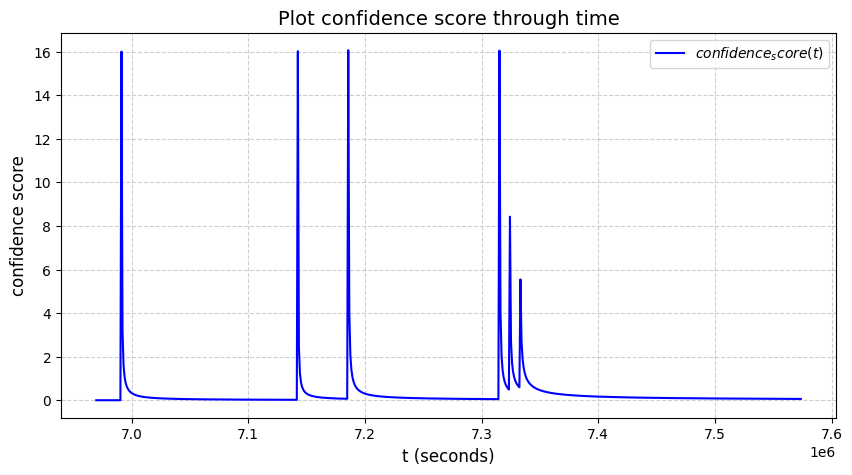
\includegraphics[width=0.75\linewidth]{confidence-score.png}
    \caption{Confidence score visualization}
    \label{fig:confidence-score}
\end{figure}

Then apply the \textit{negative exponential} to confidence\_score, we have coefficient to multiply to the recommendation score as \textbf{penalty} because it is in unit interval.

\begin{figure}[H]
    \centering
    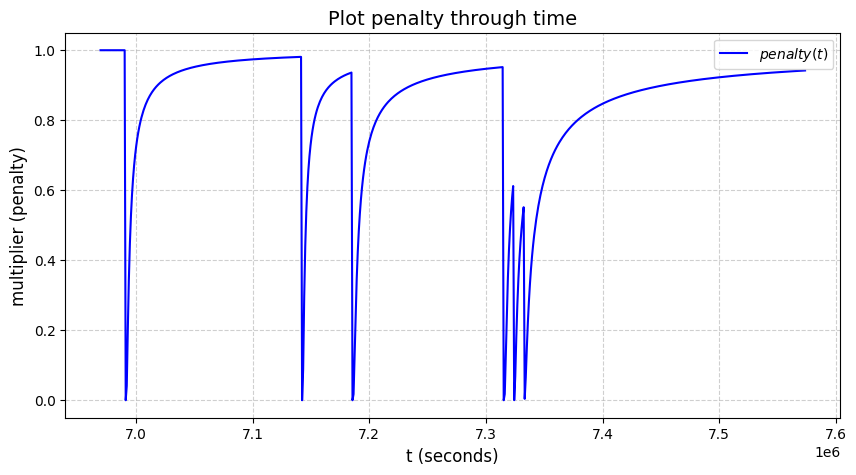
\includegraphics[width=0.75\linewidth]{penalty-multiplier.png}
    \caption{Penalty visualization}
    \label{fig:penalty-score}
\end{figure}

As depicted in the graph above, certain vertices introduce structural changes to the graph (the \textit{peaks} of graph). These vertices correspond to instances immediately following the storage of \textit{learningData} in the database. This pattern indicates that, after achieving a high performance score on a specific word, the likelihood of that word being suggested again in the near term is significantly reduced. This behavior aligns with the system's design to prioritize spaced repetition and mitigate redundant word suggestions.




\section{Algorithm} 

\subsection{Front-end}

ViteJS overcomes the disadvantages of Webpack by coming up with a wholly different concept of development and build processes. ViteJS leverages native ES Modules within modern browsers to mean that there is no need for bundling during development. With this methodology, the time taken to fire up a development server and make changes is considerably reduced. While Webpack compiles the entire dependency graph, ViteJS serves files on-demand and transforms them when needed. This leads to a nearly-instantaneous server startup and HMR that is much faster than Webpack’s implementation.

ViteJS integrates seamlessly with frameworks like React, Vue, and Svelte, commonly used in Chrome extension development. Its plugin-based architecture extends functionality and supports features like JSX and TypeScript out-of-the-box. That's the analysis for the front-end part of the application, here is the flowchart describing its algorithm:

\begin{figure}[H]
    \centering
    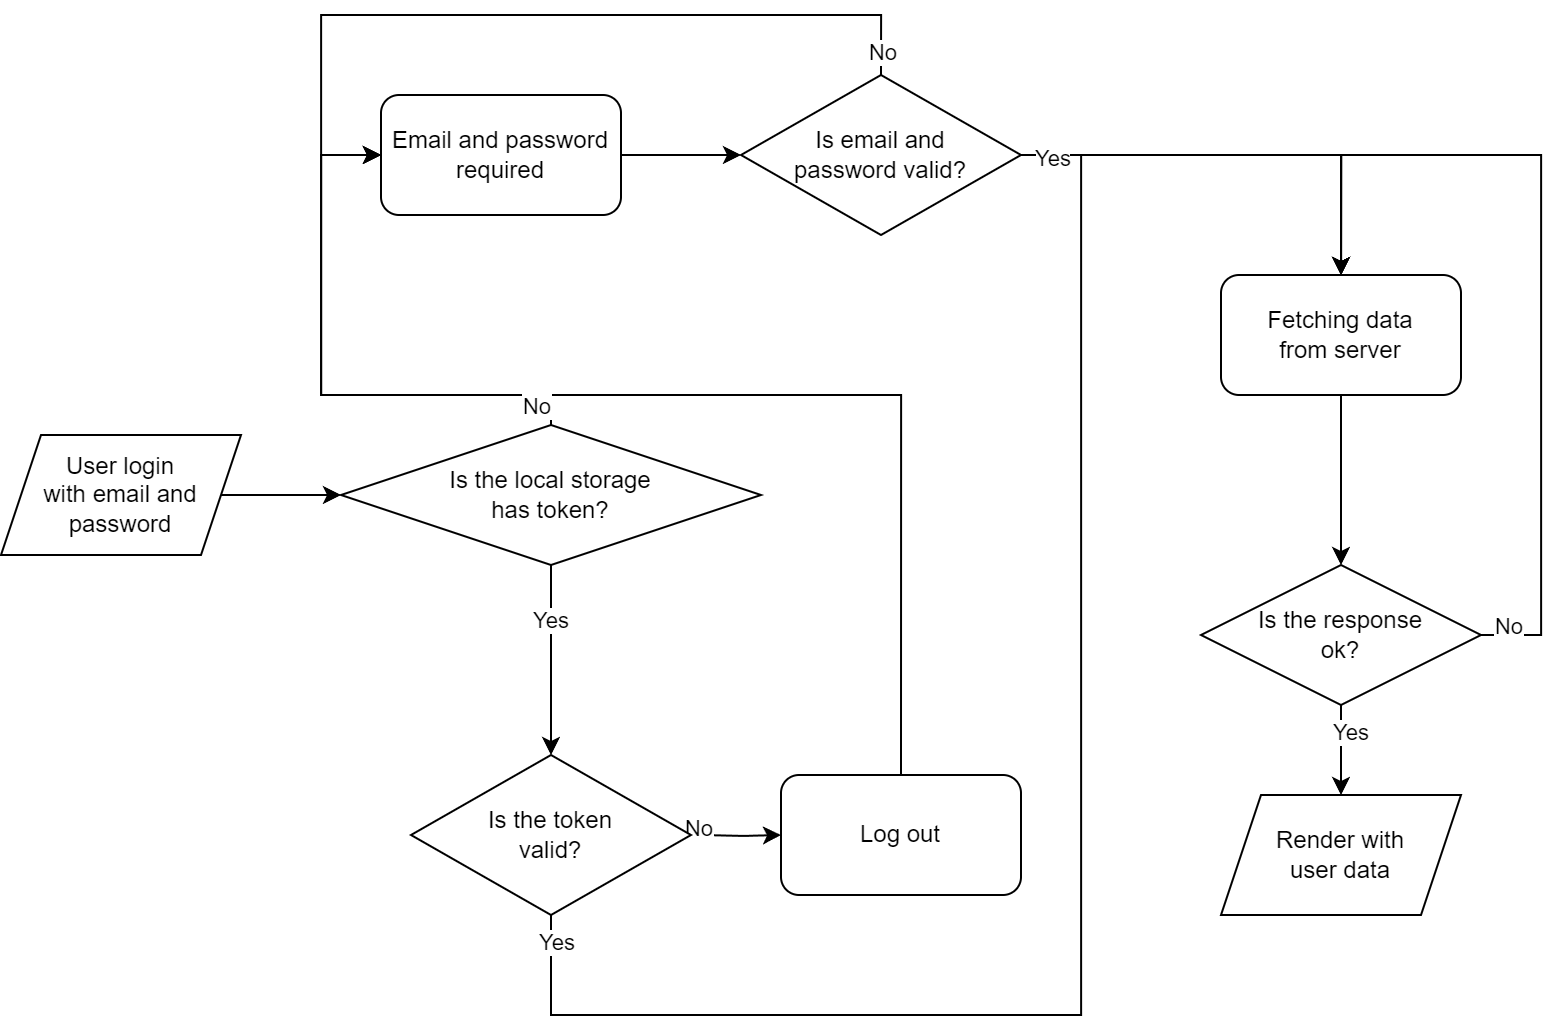
\includegraphics[width=0.75\linewidth]{flow-chart.png}
    \caption{Front-end flowchart}
    \label{fig:enter-label}
\end{figure}

\subsection{Back-end}
% \section*{Pseudocode for Feature Vector Extraction and Question Generation}
The backend architecture of the proposed English vocabulary flashcard recommendation system is designed to leverage the capabilities of FastAPI, known for its high performance and asynchronous processing, as the core backend framework. The front-end application communicates via RESTful APIs, sending requests to a NestJS middleware. NestJS acts as an intermediary layer, orchestrating the interaction between the client-side application and the backend. 

Process API requests at FastAPI, thereby ensuring the proper routing of incoming requests and handling compute-intensive tasks related to data processing and execution of the recommendation model. This architecture helps in modularity and maintenance scalability with respect to the flow of data, and though it is not mandatory, it does facilitate future enhancements. RESTful API architecture was opted for easy integration, intercoupling, and modern web standard compliance. The core aim of this project is to provide personalized recommendations on flashcards to create a user-friendly learning process.

\subsubsection{Feature Vector Calculation for Bio and Interest}
\begin{itemize}
\item Bio Feature Extraction
\begin{lstlisting}[language=Python]
Input: bio (string containing personal and professional details)
Output: bio_emb (normalized feature vector)

1. Tokenize the bio using a tokenizer.
2. Compute the text embedding of the bio using a pre-trained model.
3. Squeeze the embedding to remove unnecessary dimensions.
4. Detach the embedding from the computation graph and move it to CPU.
5. Normalize the bio_emb by dividing it by its L2 norm.
6. Return the normalized bio_emb.
\end{lstlisting}

\item Interest Feature Extraction (EMA-based)
\begin{lstlisting}[language=Python]
Input: history (list of strings containing past internet searches), 
       alpha (float, EMA parameter), previous_emb (optional, previous embedding for EMA)
Output: interest_emb (normalized feature vector for user interests)

1. Initialize interest_emb as a zero vector (1024 dimensions) if no previous_emb is provided.
2. Loop through each entry in the history:
   a. Concatenate relevant fields (e.g., title, description, keywords).
   b. Skip if the concatenated string is too short (< 50 characters).
   c. Update interest_emb using EMA:
      interest_emb = (1 - alpha) * interest_emb + alpha * text_embedding_of_entry.
3. Normalize the interest_emb by dividing it by (1 - alpha^(count+1)).
4. Return the normalized interest_emb.
\end{lstlisting}
\end{itemize}

\subsubsection{Word Similarity Computation}
\begin{lstlisting}[language=Python]
Input: WORD_EMBEDDINGS (matrix of word embeddings), WORD_MAPPING (mapping of words to indices), 
       bio_emb, interest_emb
Output: sim_bio, sim_interest (similarity scores with each word)

1. Compute the dot product between WORD_EMBEDDINGS and bio_emb to get sim_bio.
2. Compute the dot product between WORD_EMBEDDINGS and interest_emb to get sim_interest.
3. Return sim_bio and sim_interest.
\end{lstlisting}

\subsubsection{Word Frequency Calculation}
\begin{lstlisting}[language=Python]
Input: corpus (text containing all words to analyze)
Output: word_count (dictionary of word frequencies), num_words (total words in corpus)

1. Normalize the corpus by:
   a. Converting to lowercase.
   b. Replacing special characters with spaces.
   c. Splitting into words.
2. Use a Counter object to calculate the frequency of each word.
3. Return the word_count dictionary and the total word count (length of the word list).
\end{lstlisting}

\subsubsection{Score Calculation and Question Generation}
\begin{itemize}
\item Score Calculation
\begin{lstlisting}[language=Python]
Input: sim_bio, sim_interest, word_count, num_words, weights (w_bio, w_freq, w_history)
Output: final_score (list of scores for each word)

1. Initialize an empty list for final scores.
2. Loop through each word in WORD_EMBEDDINGS:
   a. Compute freq_bonus as (word frequency / total words) if the word exists in word_count; otherwise, set freq_bonus = 0.
   b. Compute the total score for the word:
      total_score = w_bio * sim_bio[idx] + w_history * sim_interest[idx] + w_freq * freq_bonus.
   c. Append the total score to the final_score list.
3. Return final_score.
\end{lstlisting}

\item Question Generation
\begin{lstlisting}[language=Python]
Input: final_score, WORD_MAPPING, k (number of questions to generate)
Output: res (list of questions with words and their answers)

1. Sort the indices of final_score in descending order of scores.
2. Select the top k indices as idx1 and the next 3k indices as idx2 (shuffle idx2 for wrong answers).
3. Initialize empty lists for word, score, and definition using idx1.
4. Loop through each word in idx1:
   a. Create a question dictionary with:
      - word_id: the word index.
      - question: the definition of the word.
      - answers: 3 wrong words (from idx2) and the correct word (shuffled).
      - correct_id: the index of the correct word in answers.
   b. Append the question dictionary to res.
5. Return the res list.
\end{lstlisting}
\end{itemize}

\subsubsection{Combining All Steps}
\begin{lstlisting}[language=Python]
Input: history, bio, corpus, WORD_EMBEDDINGS, WORD_MAPPING, k (number of questions)
Output: res (list of questions)

1. Compute interest_emb using the history and compute_interest_emb().
2. Compute bio_emb using the bio and calc_text_embedding().
3. Compute sim_bio and sim_interest using the embeddings and similarity computation.
4. Compute word_count and num_words using the corpus and word frequency count.
5. Compute final_score using the similarity scores, word frequencies, and weights.
6. Generate k questions using the final_score and question generation logic.
7. Return the res list of questions.
\end{lstlisting}


% có gì viết phần này giùm ní - oke ní 
\section{Computational Thinking Application}
The problem of recommending flashcard questions tailored to user preferences and behaviors involves significant computational thinking to ensure efficiency, accuracy, and personalization. It requires processing diverse data inputs, such as user-provided information, passive data (e.g., browser history), and interaction metrics, to generate relevant and diverse recommendations. Computational methods are essential for managing large datasets, identifying patterns, and implementing algorithms that balance constraints like diversity (high TTR) and performance. By leveraging \textit{computational thinking}, the solution integrates data processing, pattern recognition, and optimization to deliver personalized, high-quality flashcard suggestions effectively.

\begin{table}[H]
\centering
\begin{tabular}{|p{0.3\textwidth}|p{0.4\textwidth}|}
\hline
\textbf{Problem Identification} 
&
We need an English learning application that is more personalized.\\
\hline
\textbf{Pattern Recognition}
&
Users' personal information, such as career, hobbies, browsing history, and learning history, provides valuable insights for vocabulary recommendations.
\\
\hline
\textbf{Abstraction}
&
This system can effectively work by extracting features from user-provided inputs, including translations, personal information, and browser history, to generate personalized vocabulary recommendations.
\\
\hline
\end{tabular}
\caption{Iteration 1}
\label{table:ct-thinking-iter1}
\end{table}

\begin{table}[H]
\centering
\begin{tabular}{|p{0.3\textwidth}|p{0.4\textwidth}|}
\hline
\textbf{Problem Identification} 
&
What are the key requirements for the application?\\
\hline
\textbf{Pattern Recognition}
&
\begin{itemize}
\item \textit{Honesty}: Users must provide truthful information about their careers, interests, and learning preferences.
\item \textit{Access}: Users need to grant permission to access their browser history.
\item \textit{Usage}: The application should become the primary means of translation for users to collect relevant data.
\end{itemize}
\\
\hline
\textbf{Abstraction}
&
The key goal of this application is to deliver personalized vocabulary recommendations. Achieving this requires accurate and comprehensive data to best reflect the user's preferences and needs.
\\
\hline
\end{tabular}
\caption{Iteration 2}
\label{table:ct-thinking-iter2}
\end{table}

\begin{table}[H]
\centering
\begin{tabular}{|p{0.3\textwidth}|p{0.4\textwidth}|}
\hline
\textbf{Problem Identification} 
&
How can we measure the effectiveness of the system?\\
\hline
\textbf{Pattern Recognition}
&
\begin{itemize}
\item \textit{Type-Token Ratio (TTR)}: Measures the diversity of vocabulary by evaluating the proportion of unique words in a given text or user history.
\item \textit{Competence Formula}: A metric to quantify how well a user handles the recommended words, combining factors like learning success rate and familiarity with the words.
\end{itemize}
\\
\hline
\textbf{Abstraction}
&
The system needs to measure both the uniqueness of vocabulary (e.g., through TTR) and user competence (e.g., via formulas that track performance and learning progress). Recommendations should adapt to the user's evolving ability and familiarity with the language.
\\
\hline
\end{tabular}
\caption{Iteration 3}
\label{table:ct-thinking-iter3}
\end{table}

\begin{table}[H]
\centering
\begin{tabular}{|p{0.3\textwidth}|p{0.4\textwidth}|}
\hline
\textbf{Problem Identification} 
&
How can we process user-provided information, translations, and browsing history for vocabulary recommendations?
\\
\hline
\textbf{Decomposition}
&
\begin{itemize}
\item Extract user-provided information such as career, hobbies, and interests.
\item Extract insights from user translations
\item Adapt to User’s interests.
\end{itemize}
\\
\hline
\textbf{Pattern Recognition}
&
Advancements in language models like BEIT3 enable the efficient extraction of meaningful embeddings from textual data.
\\
\hline
\textbf{Abstraction}
&
The input can be framed as sentences describing the user's career, hobbies, learning goals, and browsing topics. These inputs can be used to identify and recommend vocabulary that matches the user’s context and needs.
\\
\hline
\end{tabular}
\caption{Iteration 4}
\label{table:ct-thinking-iter4}
\end{table}

\begin{table}[H]
\centering
\begin{tabular}{|p{0.3\textwidth}|p{0.4\textwidth}|}
\hline
\textbf{Problem Identification} 
&
How can we effectively extract user-provided information?\\
\hline
\textbf{Pattern Recognition}
&
\begin{itemize}
\item User-provided information is typically in sentence form, such as "I am an engineer interested in robotics."
\item BEIT3 embeddings can capture semantic meaning effectively, making it a suitable model for analyzing this input.
\end{itemize}
\\
\hline
\textbf{Abstraction}
&
User-provided information can be directly transformed into feature-rich embeddings using BEIT3. These embeddings will guide the vocabulary recommendation system.
\\
\hline
\end{tabular}
\caption{Iteration 5}
\label{table:ct-thinking-iter5}
\end{table}

\begin{table}[H]
\centering
\begin{tabular}{|p{0.3\textwidth}|p{0.4\textwidth}|}
\hline
\textbf{Problem Identification} 
&
How can we extract information from user translations?\\
\hline
\textbf{Pattern Recognition}
&
\begin{itemize}
\item \textit{Frequency of Words}: Words that appear more frequently in the user’s translations are likely more relevant to their learning process and context.
\item \textit{TF (Term Frequency) Scores}: These scores can quantify the importance of specific words within translations.
\end{itemize}
\\
\hline
\textbf{Abstraction}
&
By analyzing the frequency and term frequency of words in user translations, the system can prioritize recommending words that are more relevant and meaningful to the user.
\\
\hline
\end{tabular}
\caption{Iteration 6}
\label{table:ct-thinking-iter6}
\end{table}

\begin{table}[H]
\centering
\begin{tabular}{|p{0.3\textwidth}|p{0.4\textwidth}|}
\hline
\textbf{Problem Identification} 
&
How can we adapt to the user's interests?\\
\hline
\textbf{Pattern Recognition}
&
\begin{itemize}
\item We can utilize the Browsing history
\item Raw URLs alone do not provide enough meaningful context.
\item Extracting metadata (such as keywords, page titles, or content summaries) from URLs can provide valuable information about the user’s interests and browsing habits.
\end{itemize}
\\
\hline
\end{tabular}
\caption{Iteration 7}
\label{table:ct-thinking-iter7}
\end{table}

\section{Ethics Social}
\subsection{Privacy Problem}

The collection and processing of user information such as age, gender, occupation, interests, browsing history, and translation history pose significant challenges in ensuring data privacy and maintaining user trust. Therefore we have measures for our application for user information as follows:

\begin{itemize}
    \item \textbf{Data Minimization}: We \textit{ONLY} collect the information necessary for the functionality of the application. For example, instead of storing detailed browsing histories, consider retaining only aggregated insights that meet the application's requirements.
    \item \textbf{Explicit Consent}: We ensure users are informed about the data collected, its purpose, and how it will be used. Implement opt-in mechanisms that allow users to consent to specific data processing activities.
    \item \textbf{Consent}: Explicit user consent will be required before collecting or processing any data. Users will have the option to opt out of certain features without losing access to basic functionalities.
\end{itemize}

\subsection{Security Problem}
The backend of our application is built using NestJS, a framework renowned for its robust security features. NestJS provides a strong foundation for our application by offering built-in mechanisms for authentication, authorization, and data protection. This choice aligns with our commitment to ensuring the confidentiality and integrity of user data.
\begin{itemize}
\item 
    Authentication is a cornerstone of application security, and NestJS provides seamless integration with Passport, a widely used authentication middleware for Node.js. Passport simplifies the implementation of various authentication strategies, such as local authentication, OAuth, and third-party providers.
    
    By using Passport in NestJS, developers can implement both session-based and token-based authentication with minimal overhead, ensuring the authentication process is secure and maintainable.
\item 
JSON Web Tokens (JWT) are an industry standard for securing RESTful applications. NestJS natively supports JWT via the \textit{@nestjs/jwt package}, which works seamlessly with Passport. The JWT mechanism involves \textit{Token Issuance}, \textit{Token Validation}
\begin{figure}[H]
    \centering
    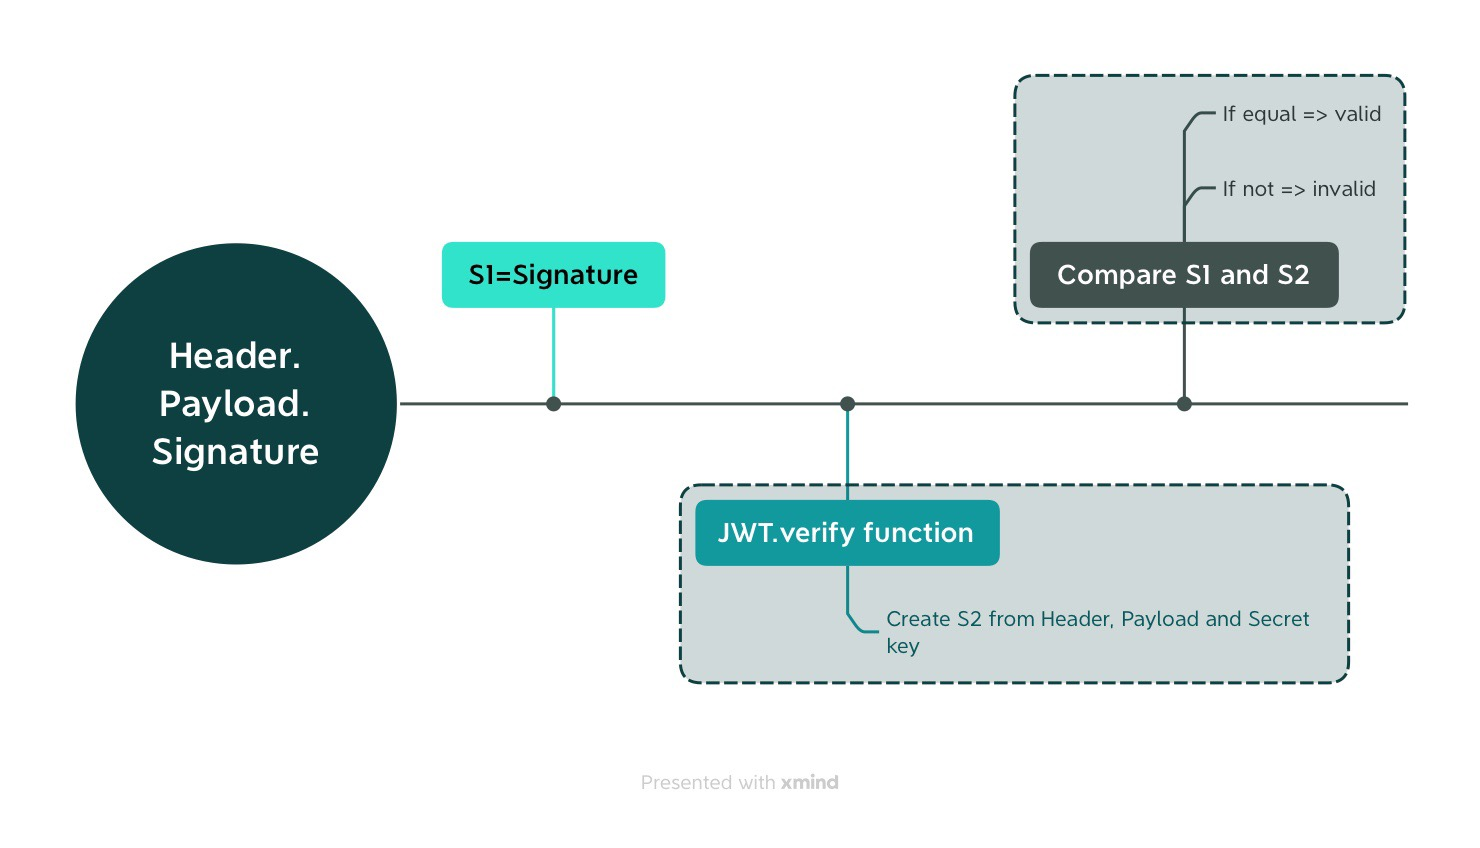
\includegraphics[width=0.75\linewidth]{jwt.png}
    \caption{JWT verify token}
    \label{fig:jwt}
\end{figure}

\item NestJS applications commonly utilize robust hashing algorithms like \textbf{bcrypt} to hash passwords before storing them in the database. These algorithms are designed specifically for password security and incorporate features such as salting and computational difficulty.

When comparing passwords, we only compare two hashed strings. Hashing is a one-way function, so if the server is attacked, the attacker will not know the user's password.
\begin{figure}[H]
    \centering
    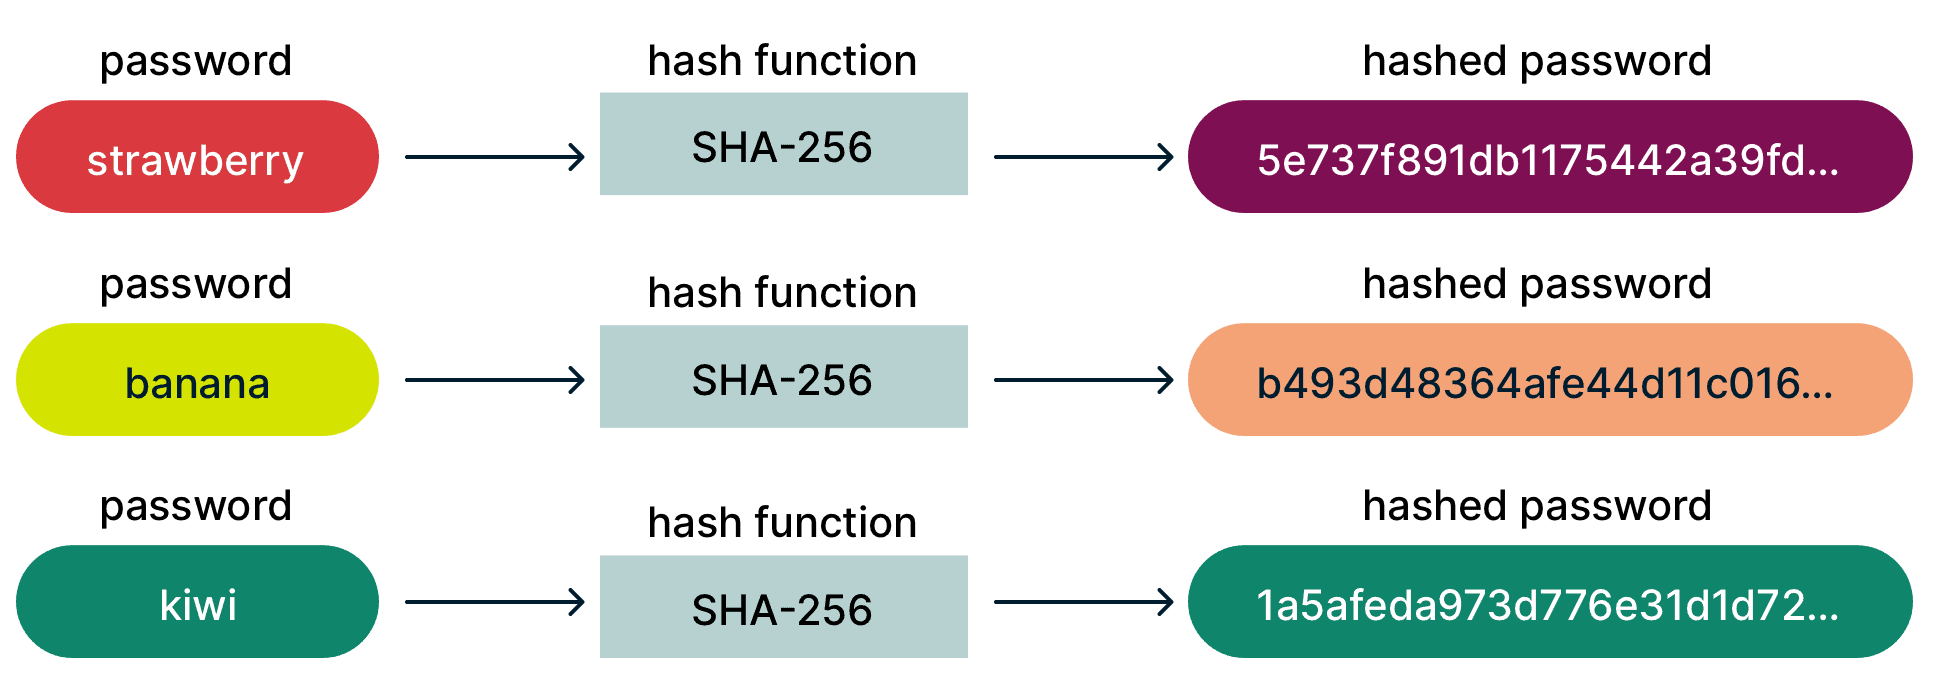
\includegraphics[width=0.75\linewidth]{hash.png}
    \caption{Hashing password}
    \label{fig:enter-label}
\end{figure}
\end{itemize}
\subsection{Copyright Problem}

The application utilizes various resources, including dictionaries, embeddings, and translations, which may involve intellectual property and copyright concerns. To mitigate these issues:
\begin{itemize}
\item 
\textbf{Licensed Resources}: Ensure that all external resources (e.g., Oxford Dictionary, Google Translate) are used in compliance with their respective licenses. Proper attribution will be provided where required.
\item 
\textbf{Fair Use Compliance}: For educational and non-commercial purposes, leverage resources under fair use guidelines. Only minimal necessary data will be utilized to achieve application objectives.
\item 
\textbf{User-Generated Content}: Clearly define user rights for content they create or provide within the application, ensuring they retain ownership of their data.
\item 
\textbf{Open-Source Models}: For models like BEIT3, adhere to the licensing terms provided by the creators to ensure no misuse of the technology.

Github repo: \href{https://github.com/trungdangtapcode/Flashcard-Recommendation-Extension}{\faGithub\ https://github.com/trungdangtapcode/Flashcard-Recommendation-Extension}




\end{itemize}

\end{document}
